
% ----------------------------------------------------------------------
%                   LATEX TEMPLATE FOR PhD THESIS
% ----------------------------------------------------------------------

% based on Harish Bhanderi's PhD/MPhil template, then Uni Cambridge
% http://www-h.eng.cam.ac.uk/help/tpl/textprocessing/ThesisStyle/
% corrected and extended in 2007 by Jakob Suckale, then MPI-CBG PhD programme
% and made available through OpenWetWare.org - the free biology wiki


%: Style file for Latex
% Most style definitions are in the external file PhDthesisPSnPDF.
% In this template package, it can be found in ./Latex/Classes/
\documentclass[twoside,11pt]{Latex/Classes/PhDthesisPSnPDF}


%: Macro file for Latex
% Macros help you summarise frequently repeated Latex commands.
% Here, they are placed in an external file /Latex/Macros/MacroFile1.tex
% An macro that you may use frequently is the figuremacro (see introduction.tex)
% This file contains macros that can be called up from connected TeX files
% It helps to summarise repeated code, e.g. figure insertion (see below).

% insert a centered figure with caption and description
% parameters 1:filename, 2:title, 3:description and label
\newcommand{\figuremacro}[3]{
	\begin{figure}[htbp]
		\centering
		\includegraphics[width=1\textwidth]{#1}
		\caption[#2]{\textbf{#2} - #3}
		\label{#1}
	\end{figure}
}

% insert a centered figure with caption and description AND WIDTH
% parameters 1:filename, 2:title, 3:description and label, 4: textwidth
% textwidth 1 means as text, 0.5 means half the width of the text
\newcommand{\figuremacroW}[4]{
	\begin{figure}[htbp]
		\centering
		\includegraphics[width=#4\textwidth]{#1}
		\caption[#2]{\textbf{#2} - #3}
		\label{#1}
	\end{figure}
}

% inserts a figure with wrapped around text; only suitable for NARROW figs
% o is for outside on a double paged document; others: l, r, i(inside)
% text and figure will each be half of the document width
% note: long captions often crash with adjacent content; take care
% in general: above 2 macro produce more reliable layout
\newcommand{\figuremacroN}[3]{
	\begin{wrapfigure}{o}{0.5\textwidth}
		\centering
		\includegraphics[width=0.48\textwidth]{#1}
		\caption[#2]{{\small\textbf{#2} - #3}}
		\label{#1}
	\end{wrapfigure}
}

% predefined commands by Harish
\newcommand{\PdfPsText}[2]{
  \ifpdf
     #1
  \else
     #2
  \fi
}

\newcommand{\IncludeGraphicsH}[3]{
  \PdfPsText{\includegraphics[height=#2]{#1}}{\includegraphics[bb = #3, height=#2]{#1}}
}

\newcommand{\IncludeGraphicsW}[3]{
  \PdfPsText{\includegraphics[width=#2]{#1}}{\includegraphics[bb = #3, width=#2]{#1}}
}

\newcommand{\InsertFig}[3]{
  \begin{figure}[!htbp]
    \begin{center}
      \leavevmode
      #1
      \caption{#2}
      \label{#3}
    \end{center}
  \end{figure}
}

\makeatletter
\def\namedlabel#1#2{\begingroup
   \def\@currentlabel{#2}%
   \label{#1}\endgroup
}
\makeatother
%%% Local Variables: 
%%% mode: latex
%%% TeX-master: "~/Documents/LaTeX/CUEDThesisPSnPDF/thesis"
%%% End: 

\usepackage[T1]{fontenc}
\usepackage{array}
\usepackage{pdfpages}
\usepackage{algorithm}
\usepackage{algpseudocode}
\usepackage{amsmath}
\usepackage[section]{placeins}
\renewcommand{\algorithmicrequire}{\textbf{Input:}}  % Use Input in the format of Algorithm
\renewcommand{\algorithmicensure}{\textbf{Output:}} % Use Output in the format of Algorithm


%\usepackage{graphics}
% or use the graphicx package for more complicated commands
%\usepackage{graphicx}

%: ----------------------------------------------------------------------
%:                  TITLE PAGE: name, degree,..
% ----------------------------------------------------------------------
\usepackage{graphicx}

      \textwidth 15cm
      \textheight 22cm
      \parindent 10pt
      \oddsidemargin 0.85cm
      \evensidemargin 0.37cm


\begin{document}

\thispagestyle{empty}

\begin{center}

Vrije Universiteit Amsterdam \hspace*{2cm} Universiteit van Amsterdam

\vspace{1mm}

\hspace*{-7.5cm}
\includegraphics[height=25mm]{0_frontmatter/figures/vu-griffioen.pdf}

\vspace*{-2cm}\hspace*{7.5cm}
\includegraphics[height=15mm]{0_frontmatter/figures/uva_logo.jpg}

\vspace{2cm}

{\Large Master Thesis}

\vspace*{1.5cm}

\rule{.9\linewidth}{.6pt}\\[0.4cm]
{\huge \bfseries Self adjusted auto provision system at resource level \par}\vspace{0.4cm}
\rule{.9\linewidth}{.6pt}\\[1.5cm]

\vspace*{2mm}

{\Large
\begin{tabular}{l}
{\bf Author:} ~~You Hu ~~~~ 2631052
\end{tabular}
}

\vspace*{2cm}

\begin{tabular}{ll}
{\it 1st daily supervisor:}   & ~~Prof. Adam Belloum ~~~~ UvA, Netherlands eScience Center \\
{\it 2nd  supervisor:} & ~~Dr. Jason Maassen ~~~~~ Netherlands eScience Center \\
{\it 2nd reader:}       & ~~supervisor name
\end{tabular}

\vspace*{2.5cm}

\textit{A thesis submitted in fulfillment of the requirements for\\ the joint UvA-VU Master of Science degree in Computer Science}

\vspace*{1.8cm}

\today\\[4cm] % Date

\end{center}

\newpage


% ----------------------------------------------------------------------
       
% turn of those nasty overfull and underfull hboxes
\hbadness=10000
\hfuzz=50pt


%: --------------------------------------------------------------
%:                  FRONT MATTER: dedications, abstract,..
% --------------------------------------------------------------


%\language{english}


% sets line spacing
\renewcommand\baselinestretch{1.2}
\baselineskip=18pt plus1pt


%: ----------------------- generate cover page ------------------------

\begin{center}
\textit{``History, as Hegel said, moves upward in a spiral of negations'' }
\end{center}

%: ----------------------- cover page back side ------------------------
% Your research institution may require reviewer names, etc.
% This cover back side is required by Dresden Med Fac; uncomment if needed.

\newpage
%\vspace{10mm}
%1. First Reader: Name Surname
%
%\vspace{10mm}
%2. Daily Supervisor: Name Surname
%
%\vspace{10mm}
%3. Second Reader: Name Surname
%
%\vspace{10mm}
%4. Industrial Supervisor: Name Surname
%
%\vspace{20mm}
%Day of the defense:

%\vspace{20mm}
%\hspace{70mm}Signature from head of PhD committee:



%: ----------------------- abstract ------------------------

% Your institution may have specific regulations if you need an abstract and where it is to be placed in the document. The default here is just after title.


% Thesis Abstract -----------------------------------------------------


%\begin{abstractslong}    %uncommenting this line, gives a different abstract heading
\begin{abstracts}        %this creates the heading for the abstract page

The resource management is no doubt one of the key problems that all cloud or cluster need to face. 
Here, the special scenario the LOFAR team is taking: they build computation infrastructure of their own to process the data collected by the tremendous telescopes.
They are both cloud provider and cloud user. The jobs the cloud is undertaking are long and highly computation consuming.
The current horizontal distributed solutions, MPI and Spark, have intrinsic drawback on resource utilizing. 
To increase the resource utilization level, an auto-provisioning distributed computing system is designed. 
The auto-scaling mechanism enables the applications to dynamically fetch and release resources, and in the same time the resources of the cluster are maximally used.
The results shows:% TODO: add results and conclusions


\end{abstracts}
%\end{abstractlongs}


% ---------------------------------------------------------------------- 


% The original template provides and abstractseparate environment, if your institution requires them to be separate. I think it's easier to print the abstract from the complete thesis by restricting printing to the relevant page.
% \begin{abstractseparate}
%   
% Thesis Abstract -----------------------------------------------------


%\begin{abstractslong}    %uncommenting this line, gives a different abstract heading
\begin{abstracts}        %this creates the heading for the abstract page

The resource management is no doubt one of the key problems that all cloud or cluster need to face. 
Here, the special scenario the LOFAR team is taking: they build computation infrastructure of their own to process the data collected by the tremendous telescopes.
They are both cloud provider and cloud user. The jobs the cloud is undertaking are long and highly computation consuming.
The current horizontal distributed solutions, MPI and Spark, have intrinsic drawback on resource utilizing. 
To increase the resource utilization level, an auto-provisioning distributed computing system is designed. 
The auto-scaling mechanism enables the applications to dynamically fetch and release resources, and in the same time the resources of the cluster are maximally used.
The results shows:% TODO: add results and conclusions


\end{abstracts}
%\end{abstractlongs}


% ---------------------------------------------------------------------- 

% \end{abstractseparate}


%: ----------------------- tie in front matter ------------------------

\frontmatter
% Thesis Dedication ---------------------------------------------------

%\begin{dedication} %this creates the heading for the dedication page

%To ...

%\end{dedication}

% ----------------------------------------------------------------------
% Thesis Acknowledgements ------------------------------------------------


%\begin{acknowledgementslong} %uncommenting this line, gives a different acknowledgements heading
%\begin{acknowledgements}      %this creates the heading for the acknowlegments


%\end{acknowledgements}
%\end{acknowledgmentslong}

% ------------------------------------------------------------------------





%: ----------------------- contents ------------------------

\setcounter{secnumdepth}{3} % organisational level that receives a numbers
\setcounter{tocdepth}{3}    % print table of contents for level 3
\tableofcontents            % print the table of contents
% levels are: 0 - chapter, 1 - section, 2 - subsection, 3 - subsection


%: ----------------------- list of figures/tables ------------------------

\listoffigures	% print list of figures

\listoftables  % print list of tables




%: ----------------------- glossary ------------------------

% Tie in external source file for definitions: /0_frontmatter/glossary.tex
% Glossary entries can also be defined in the main text. See glossary.tex
% 
%% this file is called up by thesis.tex
% content in this file will be fed into the main document

% Glossary entries are defined with the command \nomenclature{1}{2}
% 1 = Entry name, e.g. abbreviation; 2 = Explanation
% You can place all explanations in this separate file or declare them in the middle of the text. Either way they will be collected in the glossary.

% required to print nomenclature name to page header
%\markboth{\MakeUppercase{\nomname}}{\MakeUppercase{\nomname}}


% ----------------------- contents from here ------------------------


%\nomenclature{LSY}{ehbfuefebbfbjkjkebfjbfbfw} 
%\nomenclature{DEPC}{diethyl-pyro-carbonate; used to remove RNA-degrading enzymes (RNAases) from water and laboratory utensils}
%\nomenclature{DMSO}{dimethyl sulfoxide; organic solvent, readily passes through skin, cryoprotectant in cell culture}
%\nomenclature{EDTA}{Ethylene-diamine-tetraacetic acid; a chelating (two-pronged) molecule used to sequester most divalent (or trivalent) metal ions, such as calcium (Ca$^{2+}$) and magnesium (Mg$^{2+}$), copper (Cu$^{2+}$), or iron (Fe$^{2+}$ / Fe$^{3+}$)}



 

%\begin{multicols}{2} % \begin{multicols}{#columns}[header text][space]
%\begin{footnotesize} % scriptsize(7) < footnotesize(8) < small (9) < normal (10)

%\printnomenclature[1.5cm] % [] = distance between entry and description
%\label{nom} % target name for links to glossary

%\end{footnotesize}
%\end{multicols}



%: --------------------------------------------------------------
%:                  MAIN DOCUMENT SECTION
% --------------------------------------------------------------

% the main text starts here with the introduction, 1st chapter,...
\mainmatter

\renewcommand{\chaptername}{} % uncomment to print only "1" not "Chapter 1"


%: ----------------------- subdocuments ------------------------

% Parts of the thesis are included below. Rename the files as required.
% But take care that the paths match. You can also change the order of appearance by moving the include commands.


% this file is called up by thesis.tex
% content in this file will be fed into the main document
%: ----------------------- introduction file header -----------------------
\chapter{Introduction}

% the code below specifies where the figures are stored
\ifpdf
    \graphicspath{{1_introduction/figures/PNG/}{1_introduction/figures/PDF/}{1_introduction/figures/}}
\else
    \graphicspath{{1_introduction/figures/EPS/}{1_introduction/figures/}}
\fi

% ----------------------------------------------------------------------
%: ----------------------- introduction content ----------------------- 
% ----------------------------------------------------------------------



%: ----------------------- HELP: latex document organisation
% the commands below help you to subdivide and organise your thesis
%    \chapter{}       = level 1, top level
%    \section{}       = level 2
%    \subsection{}    = level 3
%    \subsubsection{} = level 4
% note that everything after the percentage sign is hidden from output



\section{Context} 
The LOw Frequency Array(LOFAR) telescope\footnote{\url{http://www.lofar.org/}} demands for huge data processing ability. 
It consists of 51 stations cross Europe and a typical LOFAR observation has the size of 100TB, after frequency averaging, the size can be reduced to 16TB. \cite{Spreeuw2019}
Collectively, there are over 5 PB of data will be stored each year. \cite{Start2020} In the data processing pipeline, the image calibration is a vital step. 
As the data collecting speed exceeds the capability of processing, the data will be stored and archived first. It will be feed to processing pipeline when it is needed.
The Netherlands eScience Center has developed solutions for calibrating imaged observation collected by LOFAR. The one of the way is sky map based direction independent calibration.
To calibrate the observation by given sky map, SAGECaL is invented and implemented for this purpose.\cite{Kazemi2011}. 
By given pre-processed observation data, sky model and parameters, the calibration can be done independently. 
However, it is a computation consuming application. Currently, eScience Center has developed GPU, MPI and Spark versions for acceleration.
All of them have achieved great acceleration compared to the naive uni-node version. 

However, under the huge requirement of computation, all three solutions have limitation. The GPU version provide no doubly great acceleration, which is in a sense vertical scaling.
MPI and Spark can be considered as horizontal scaling, GPU can provide support as well. But as it is said, LOAFR is cloud user and cloud provider in the same time, the resource utilization of their infrastructure is also important.
The MIP and Spark solutions may lead to waste of resources. The Fig. \ref{fig:sparkUti} gives an example that when the required computation resources decrease, idle resources(compute nodes) wouldn't be released by Spark.
On the other hand, a pure batch job system may enter a very special situation that a big job is waiting for resource while idle resources can not fulfill the requirement, for instance as shown in Fig. \ref{fig:MPIUti}.


% \begin{figure}
%     \centering
%     \begin{minipage}
%         \figuremacroW{1_introduction/figures/spark_NP.jpg}{Spark}{Spark occupys fixed resources}{0.45}
%     \end{minipage}
%     \begin{minipage}
%         \figuremacroW{1_introduction/figures/spark_NP.jpg}{Spark}{Spark occupys fixed resources}{0.45}
%     \end{minipage}
% \end{figure}

\begin{figure}
    \centering
    \begin{minipage}{.5\textwidth}
      \centering
      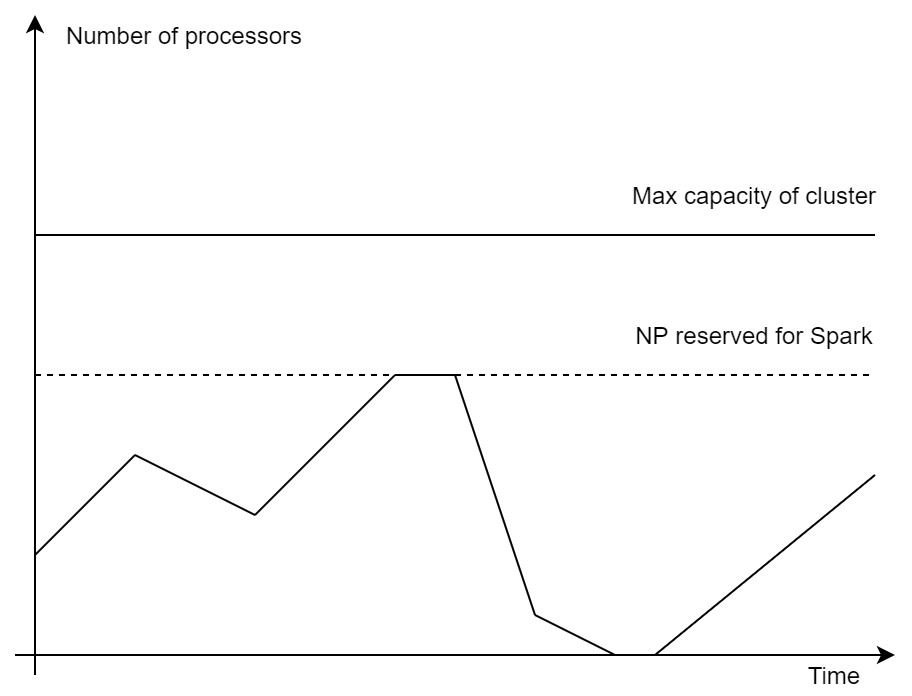
\includegraphics[width=0.9\linewidth]{1_introduction/figures/spark_NP.jpg}
      \caption[SparkUti]{{\small\textbf{Resource utilization by Spark} - Spark occupys fixed resources}}
      \label{fig:sparkUti}
    \end{minipage}%
    \begin{minipage}{.5\textwidth}
      \centering
      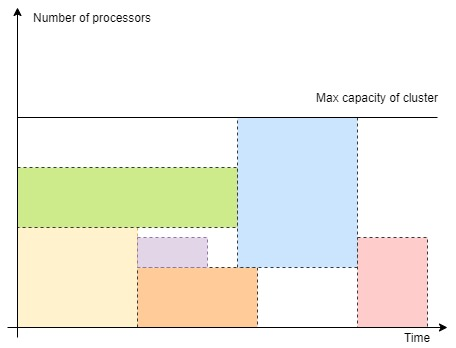
\includegraphics[width=0.9\linewidth]{1_introduction/figures/MPI_batch.jpg}
      \caption[MPIUti]{{\small\textbf{Resource utilization by MPI} - Too large jobs make resource waste}}
      \label{fig:MPIUti}
    \end{minipage}
\end{figure}
% \figuremacroW{1_introduction/figures/spark_NP.jpg}{Spark}{Spark occupys fixed resources}{0.45}
% \figuremacroW{1_introduction/figures/spark_NP.jpg}{Spark}{Spark occupys fixed resources}{0.45}
% \begin{figure}[htbp]
%     \centering
%     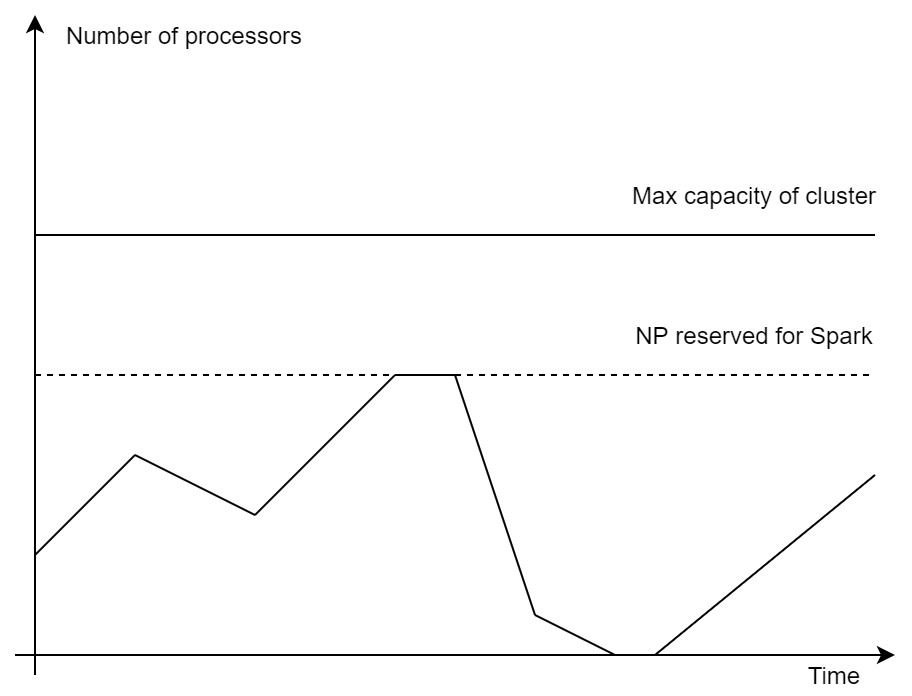
\includegraphics[width=\textwidth]{1_introduction/figures/spark_NP.jpg}
%     \caption[123]{123}
%     \label{134}
% \end{figure}

\section{Objective}

In the previous section, it is mentioned that LOAFR team has the role of both sides. Therefore, in this research, higher resource utilization of cloud system is the first objective.
In the same time, the acceleration of calibration processing is the second goal to achieve. Hopefully, the higher resource utilization, or in other words more active computation resources, is able to shrink the time for computing.

\section{Research Question}
The research question overall is how to implement an elastic distributed algorithm that can be auto-scaled dynamically that reduces the waste of resources.
More particularly, it can be extended into more specific questions:
\begin{itemize}
  \item How to set up an auto provisioning system adopting to the workload of a cloud that requests and releases resources dynamically?
  \item How to transform the calibration application into distributed and parallel version?
  \item How to make the distributed application capable to the dynamic scaling environment?
\end{itemize}


\section{Research Method}
The research method is practice based implementation plus comparison. 
In this research, firstly the previous work and current solutions will be explored. The limit, pros and cons of previous work will be collected and analyzed.
Secondly, a system that fulfills the demand of auto provisioning and overall higher resource utilization will be implemented.
Last, the system will be tested by given benchmark, and compared to other systems on the objective goals.

 


% this file is called up by thesis.tex
% content in this file will be fed into the main document

\chapter{Technical backgrounds} % top level followed by section, subsection


% ----------------------- paths to graphics ------------------------

% change according to folder and file names
\ifpdf
    \graphicspath{{2_literaturereview/figures/PNG/}{2_literaturereview/figures/PDF/}{2_literaturereview/figures/}}
\else
    \graphicspath{{2_literaturereview/figures/EPS/}{2_literaturereview/figures/}}
\fi


% ----------------------- contents from here ------------------------
% 
In this chapter, we will firstly go in to the detail for two implementations of LOAFR pipeline made by eScience center.
And then, we will briefly describe resource management techniques in HPC clusters, focusing on high resource utilization for cluster computing environment.
The batch scheduling has a long history covering the entire computer systems field from the mainframe age, up to today computing systems. Batch scheduling is still default scheduling method for modern computer systems. 
The simple FIFO batch scheduling systems turned to be quite inefficient  and a number of optimization were proposed like Preempting, backfill, and heuristics.
In the following sections, we will explore these kinds of solutions respectively 
%-----------------------------overview-----------------------------------
\section{Existing solutions}
\subsubsection*{MPI version}
SAGECaL native supports multi-threads parallelization and GPU. The MPI version of SAGECaL\footnote{\url{https://github.com/nlesc-dirac/sagecal/tree/master/src/MPI}} employs a master/worker architecture to manage the task distribution among nodes.
The task division is based on the data partitioning. Each worker node process a file at a time. 
The master tries to equally distribute tasks, but the work load can not be adjusted during the runtime.
Besides, this MPI version does not support fault tolerance in case worker nodes fail during the processing.
\subsubsection*{Spark version}
To make better use of resources, eScience center also developed a spark version of SAGECaL\footnote{\url{https://github.com/nlesc-dirac/sagecal-on-spark/tree/master/excon/JAVA}}.
The SAGECaL is compiled as dynamic library and utilized by Java native interface. The tasks are divided by file as well, and are managed by Spark. 
Compared to MPI version, Spark provides better resource management and fault tolerance. 
Besides, with the help of container technology and container orchestras like Kubernetes, we can scale the running Spark environment manually.
\section{System dependency}
\subsection{SLURM}
SLURM, formerly known as Simple Linux Utility for Resource Management, is a cluster management and job scheduling system for large and small Linux clusters1 which is
open-source, fault-tolerant, and highly scalable. There are three critical functions, as it
is stated, that is, allocating resources to users for a duration of time, providing a job
management framework over-allocated node, and arbitrating contention for resources by
a queue. SLURM can be configured with multiple kinds of queuing strategies, by default
backfilling set up to maximize resource utilization in universal cases.

In our project, the scaling relies on the submission and cancellation of jobs. To
make a decision, the status of the cluster will also be periodically collected. The status
includes the resource occupation and information of jobs in the queue. According to
these statuses, the resource manager makes decisions to scale the calibration jobs. The
SLURM receives instructions from Resource manager of our system and allocates/retrieves
resources by commands. And in the same time, it provides status of the cluster to the
Resource manager.

\subsection{Xenon}
Xenon\footnote{\url{https://xenon-middleware.github.io/xenon/}}, a middleware abstraction library, is utilized to manage the information and resources in an organized way, which enables our resource managers to communicate with the cluster in a more robust way, instead of parsing the output of command lines. 
It is designed for simple access to distributed computing and storage resources, which provides a single programming interface to many types of remote resources. 
\subsection{Shared file system}
One of the fundamental requirements for this system lies in the shared file system which
allows us to achieve fault tolerance in a simple way. The shared file system can be accessed
by all nodes, including head node and work nodes. It stores the container images of modules
and processing environment for different kinds of jobs. The executors will read the raw
data obtained from it, and generate result which will be sent back.

\section{Traditional resource management strategies}
\subsection{Preemption based resource management systems}
Preemption is usually used to avoid job delaying and resources starvation. 
Furthermore, apparently, resuming the execution of  preempted jobs is the most time-consuming part. 
At the resources level, the preemption strategy is not common to be directly used on job scheduling along, instead, it is combined with other additional techniques. 
Sajjapongse et al. \cite{sajjapongse2013preemption} proposed a run- time system based on a preemption strategy to increase GPU utilization on heterogeneous clusters. 
The paper describes the performance of hybrid MPI-CUDA applications showing the efficiency of preemption based mechanisms. 
To overcome the drawbacks related to preemption, including the waste of resources, many adaptions are proposed. 
Lu Cheng et al. \cite{6103959} proposed a solution inspired from Mapreduce. 
They introduced a component Global Preemption to trade short-term fairness for better efficiency. 
Another way approach is the checkpoint/restart mechanisms used by Berkely lab\cite{hargrove2006berkeley} in their Linux cluster. 
However, in the real environment, people use preemption strategies very carefully. 
Unless all jobs are equipped with a caching mechanism, otherwise, the cost of canceling running jobs will be unaffordable.

\section{Backfill based resource management systems}
The backfill algorithm is currently the default schedule algorithm to achieve as high resource utilization  in production environment, which gives small jobs a higher priority. 
In Section \ref{sec:backfill}, a backfill algorithm will be addressed in detail. 
Suresh et al. used a balanced spiral method for cloud metaschedules\cite{5972255}, which improves the performance and, at the same time, meets the requirement of QoS requirement of cloud systems.  
While Nayak et al. proposed a novel backfilling-based task scheduling algorithm to schedule deadline-based tasks\cite{nayak2019dynamic}. 
It aims to break the performance limit of the default backfilling algorithm of OpenNebula. 
This VM-based solution achieved minor improvement of resource utilization. 
Backfilling scheduling shows great generic and ability for using resource utilization.

A number of variations of the backfill technique have been proposed for different system configurations.
EASY-backfill and conservative backfill hold the restriction not delay the job ahead\cite{4797220}.
EASY-backfill is more aggressive, that is, for any job pending in the queue, backfill happens only when a small job does not delay the job at the head of the queue. 
However, in conservative setting, a job’s backfill requires that the filling does not delay any job before it. 
Additionally, Flexible\cite{talby1999supporting} and Multi-queue backfilling\cite{lawson2002multiple} are proposed to meet the requirements of more dynamic scenarios, and reduce the response time for some jobs. 
Flexible tries to introduce slack factor to rise the priorities of big jobs in the queue. For multi-queue backfill, the partition will adapt as the workload change.

However, in terms of resource utilization, this algorithm still has some performance limitations, if there is no job that requires fewer processors than free processors, the free processors will remain idle. 
In \cite{hafshejani2013efficient}, Hafshejani et al. turned to schedule jobs on thread instead of on processor. 
They tried to improve the resource utilization via finer-granularity allocation. 
The results show that less response time on average is achieved compared with FCFS and traditional Backfilling.
 
\section{Resource management stratgies in research}
\subsection{Heuristics}
Heuristics algorithms are usually more efficient, which take less time to decide as scheduling problem is NP-Hard. 
Xhafa and Abraham did a survey\cite{xhafa2010computational} and explored the application of heuristics algorithms in job scheduling. 
The most common and straightforward approach is local search, and the methods in this family include Hill Climbing (HC), Simulated Annealing (SA), and Tabu Search (TS), etc. 
In \cite{ritchie2003fast}, local search facilitates the shortening of  schedule on benchmark problems. 
Though the population-based approaches are more efficient, they require a longer time to convergence. 
In \cite{abraham2000nature}, the Genetic Algorithm approach allows the sufficient utilization of the resources. 
Moreover, of course, in this work, the above two approaches show that they can be combined to achieve a better performance. 

\subsection{Machine learning}
The machine/deep learning was greatly improved during the last few years, a couple of recent studies applied ML/DL approaches to resource  management.  Research made by Mao et al.\cite{mao2016resource} shows that (deep)reinforcement learning is able to outperform the  traditional state-of-art approaches. 
It translates the problem of packing tasks with multiple resources (herein referred to CPU and memory) demands into a learning problem. 
Another similar study\cite{8622393} also shows that the RL-based approach has great potential for resource management. 
However, the approach was only tested in simulation with synthetic load generated using well known probability distribution like Bernoull process, Uniform distribution, and Beta distribution. 

ML/DL techniques have also been used to improve more traditional resource management algorithm.
For instance, Gaussier et al.\cite{7832838} used machine learning to improve backfilling. 
Backfill strategy relies on the estimated execution time which is normally assigned by users. Through predicting the execution time, better by ML model, backfill mechanism is available to make better decisions.



% ---------------------------------------------------------------------------
% ----------------------- end of thesis sub-document ------------------------
% ---------------------------------------------------------------------------
	
% this file is called up by thesis.tex
% content in this file will be fed into the main document

\chapter{Backfilling and scaling policy}\label{chapter:4-1} % top level followed by section, subsection

\ifpdf
    \graphicspath{{3_methods/figures/PNG/}{3_methods/figures/PDF/}{3_methods/figures/}}
\else
    \graphicspath{{3_methods/figures/EPS/}{3_methods/figures/}}
\fi

In this chapter, we first explain the backfill mechanism in more detail. 
Then we will describe a specialized scaling policy to maximize resource utilization . 

\section{Backfill mechanism}\label{sec:backfill}
The backfill scheduling plug-in is loaded by default in the SLURM cluster. 
In the previous chapter, we have listed a few works related to backfill policy. 
Therefore, currently, we only consider the dynamic provision of CPU resources via SLURM job submission/canceling.
By the setting of job submission and canceling, we designed the scaling policy of the resource manager to adapt to the backfill mechanism.

As an optimization for the basic priority queue, the backfilling scheduling starts the lower priority jobs provided it does not delay the expected start time of any higher priority jobs. 
In other words, the backfilling mechanism under discussion refers to the conservative backfill because standard configurations of clusters using in research aim to achieve a fair share of the computing resource among the users.
An intuitive interpretation is shown in Fig. \ref{fig:backfillCas} and Fig. \ref{fig:backfillCase}.

\begin{figure}[!h]
    \centering
    \begin{minipage}{.45\textwidth}
      \centering
      \includegraphics[width=1\linewidth]{3_methods/figures/backfilling1.png}
      \caption[Backfill case 1]{{\small\textbf{Job 5 is backfilled} - Job 4 is estimated to start after the finishing of Job 2}}
      \label{fig:backfillCas}
    \end{minipage} 
    \begin{minipage}{.45\textwidth}
      \centering
      \includegraphics[width=1\linewidth]{3_methods/figures/backfilling2.png}
      \caption[Backfill case 2]{{\small\textbf{Job 7 is backfilled} - Running Job 7 will not impact Job 4 and Job 6 }}
      \label{fig:backfillCase}
    \end{minipage}
\end{figure}
According to the configuration of SLURM, the backfilling scheduling is triggered when jobs are submitted/finished. 
Besides, the scheduler periodically checks whether a job in the queue is available to run.
The decisions for backfilling depend on the number of resources, and the time limits of the jobs. 

As shown in  Fig. \ref{fig:backfillCas}, Job 4 is pending in the queue due to the lack of resources.
When Job 5 is appended to the queue, the scheduler estimates that Job 5 can be finished before Job 4 gets adequate resources. 
Therefore, the resource is allocated to Job 5.

Another scenario is shown in Fig. \ref{fig:backfillCase}. Job 7 is added to the queue while it requires minimal resources, which will last when Job 4 is on the run by the estimation. 
Besides, it still gets the assigned resource as it does not affect the jobs ahead of it(by the estimation of starting time and priority).

The typical cases above show how the backfill mechanism works. 
In practice, the scheduler considers pending jobs in priority orders, that is, once a pending job fulfills the requirements of the backfill condition, it can start immediately. 
The resource manager of our system employs an adaptive algorithm that utilizes the backfilling mechanism to achieve high resource utilization.

\section{An approach to maximize resource utilization}
In the previous section, we discussed how backfilling mechanism enlarges resource utilization.
In the default setting, users may submit any kind of job. 
However, in some cases like LOFAR use case, the users may execute the same program for different datasets.
Therefore, we propose a resource management system that reorganizes one or more kinds of job execution and manages resources in a dynamic way.
The system can retrieve and release resources according to scaling policy so that the overall resource can be fully used.
\section{Scaling policy}
The scaling policy aims to harvest every idle resource,  which requires continuous monitoring of the status of the cluster and the running or pending jobs. 
The resource manager periodically fetches status information, and makes decisions based on a scaling algorithm which acts according to the following figures:
\begin{itemize}
    \item $I$ - The number of idle nodes in a (partition of) cluster
    \item $T$ - The total number of nodes in a (partition of) cluster
    \item $R$ - The number of nodes reserved for our system
    \item $J_{i}$ - The pending or running job with ID $i$  
    \item $N_{i}$ - The number of required nodes of $J_{i}$
    \item $TL_{i}$ - The time limit of $J_{i}$
    \item $RT_{i}$ - The running time of $J_{i}$
    \item $MiniNode$ - The minimum number of nodes reserved for our system
\end{itemize}

In the following, we demonstrate three cases that explain what will happen under the given conditions. 
Note that we describe background jobs as $Job i$ which are submitted by other users.
At the same time, we will name The resources reserved for our system as $Calibration$ as we will use the LOFAR calibration pipeline as the test use case.

\subsection{Case 1: RM harvest idle resources }
First, considering that sometimes there is no job pending in the queue, there are $I$ nodes remaining idle.
To increase the overall resource utilization, the resource manager will submit $I$ one-node jobs, thereby sharing the calibration application workload, which is the basic strategy for any auto-scaling system. 
The distributed jobs will be accelerated, benefiting from more resources allocated.

\subsection{Case 2: RM give free resources}
To be friendly with other users, the system release resources when it gets sufficient resources($R>=MiniNode$), and other jobs are pending.
In the case that the extra part of resources exceeds the requirement of the first pending job, resources will be released in our case from the set of resources needed for the LOFAR Calibration application.
In other words, the system is trying to let as many jobs as possible run, provided that the giving out of resources will not slow down the calibration application($R<MiniNode$).
\textbf{Example:}

At a time, the resource manager collected the information from the cluster and jobs.
Let $T=21$,$MiniNode=10$. And there two jobs $J_{1}$ and $J_{2}$ are running, where $N_{1}=5$, $N_{2}=5$, $TL_{1}=20 min$ and $TL_{2}=15 min$.
Assume that both $RT_{1}$ and $RT_{2}$ are equal to $1 min$. And there are two pending jobs $J_{3}$ and $J_{4}$ with  $N_{3}=10$, $N_{4}=6$, $TL_{3}=25 min$ and $TL_{4}=10 min$.
Now, the system has taken the rest 11 nodes in the cluster, which means $R=11$.
If $J_{2}$ is canceled somehow, then $I=5$. It is easy to find that if the resource manager shares one more node, plus five idle nodes, $J_{6}$ can start according to the backfilling policy. 
After that, $R$ is still not less than $MiniNode$. A graphic illustration is displayed in \ref{3_methods/figures/backfillingCase2.jpg}, where the dotted line represents the number of $MiniNode$. 
\figuremacroW{3_methods/figures/backfillingCase2.jpg}{Scaling policy Case 2}{$J_{2}$ canceled, the system gives way, $J_{4}$ is backfilled }{1}
Please be noted that if the job on top of the queue, herein refers to  $J_{3}$, is able to start once getting sufficient resources, the resource manager will give way for it. And in the implementation, the job on the head of the queue will be considered first, which is followed by the jobs behind.

\subsection{Case 3: RM does not free resources }

The prerequisite of giving way for other jobs is that giving out resources would not break down the $MiniNode$, and the time limit is appropriate.
In the case that there are no suitable jobs available to be backfilled, the resource manager takes those idle resources.
It first calculates the maximum time necessary to ensure that a job can be backfilled. If no job can be backfilled, the resource manager submits $I$ one-node jobs with $TL=maxTime-2mins$.
The reason to subtract 2 minutes is to ensure that the jobs can be backfilled correctly so that we make them redundant.
The backfilling scheduling takes a long time, especially when there are many jobs on the cluster(running and pending).

\textbf{Example:}

The setting and jobs are the same as the previous example, however, we changed the time limit of J4 to 25 minutes.
Thus, the resource manager submits jobs with $TL=17 mins$ to take 5 idle nodes. This scenario is illustrated in Fig. \ref{3_methods/figures/backfillingCase3.jpg}.

\figuremacroW{3_methods/figures/backfillingCase3.jpg}{Scaling policy Case 3}{$J_{2}$ canceled, calibration application takes the idle resources because backfilling $J_{4}$ will delay $J_{3}$. Then calibration application takes them }{1}


% ----------------------- paths to graphics ------------------------

% change according to folder and file names
\ifpdf
    \graphicspath{{3_methods/figures/PNG/}{3_methods/figures/PDF/}{3_methods/figures/}}
\else
    \graphicspath{{3_methods/figures/EPS/}{3_methods/figures/}}
\fi


% ----------------------- contents from here ------------------------
% 


%-----------------------------overview-----------------------------------

\chapter{Architecture and implementation}\label{chapter:4} % top level followed by section, subsection

\section{Overview design}
Based on the review of the previous works and the scaling policy described in previous chapter, a system is proposed for the research questions: a user-side solution for overall resource utilization of batch job clusters.
The system consists of two layers, i.e., the management layer and the computation layer. The overview design is illustrated in Fig.\ref{3_methods/figures/SimpleLayers.jpg}. 
At the management layer, the resource layer is responsible for deciding resource allocation at runtime; 
therefore, the computation layer is enabled to scale on demand, which is responsible for parallel job execution. 
The computation layer is composed of multiple executors on arbitrary working nodes by the demand. 
All nodes can access the shared file system which is provided by the cluster. 
In the following sections, we first explain the functionality of each component and how these components interact with each other. 
And then, we explore the detailed implementations of this system.

\begin{figure}
  \centering
  \includegraphics[width=0.75\linewidth]{3_methods/figures/SimpleLayers.jpg}
  \caption[Layers and components]{Three components are placed in two layers with a shared file system at button}
  \label{3_methods/figures/SimpleLayers.jpg}
\end{figure}

\section{Components}
\subsection{Resource manager}
The Resource Manager(RM) is mainly responsible for deciding to change the number of resources allocated to this system. 
The decision-making is based on the information obtained from SLURM and WebService. 
The RM continuously queries the status of the available resources via the Xenon interface.

Besides, the RM also fetches information about the status of users’ jobs from WebService(Web server in Fig.\ref{3_methods/figures/SimpleLayers.jpg}) through Restful API. 
These statistics help the resource manager to make decisions.

\subsection{Service module}
Consisted of two sub-components, the service module is a container instance hosting a web server and an Ibis server. 
In this project, we assume that the head node never crashes, and the processes are not terminated by external action.

The web server is based on Flask Restful framework. The end-users can submit jobs via Restful API, and the webserver temporally stores the configuration of those jobs. 
Besides, this webserver also allows the master of executors to update the recommended minimal working nodes. 
This number can be used for RM to make scaling decisions. 
Note that the term job herein refers to application-related jobs. The other server is the Ibis server. In the computation layer, Ibis Portability Layer(IPL)\cite{5492667} is employed for communication. 
The IPL requires an Ibis server as a centralized hub for managing the communication and events among Ibis instances. 
Considering the requirement for stabilization, we choose to run the Ibis server on the head node to mitigate the risk of crashing.
 
\subsection{Executors}
The executors are the main power for data processing. 
In this project, every time RM decides to scale up the computation ability of the system, it will submit a new pre-defined job to SLURM. 
Once this job is executed, a new executor is added to the pool of application executors.

By exploiting IPL interfaces, the computation layer is designed as shown in Fig. \ref{3_methods/figures/computingModel.png}. 
Every executor creates an Ibis instance for communication, and all the instances, after initialization, will poll an election to select the master. 
As a result, one executor is acting as the master and the rest of the executors are tasked with processing the data.
In our project, the executors process data based on containers, which enables our system to handle multiple types of jobs for different kinds of data set.

\begin{figure}
  \centering
  \includegraphics[width=1\linewidth]{3_methods/figures/computingModel.png}
  \caption[Distributed computing model]{Master-worker architecture, red boxes indicate the batch size}
  \label{3_methods/figures/computingModel.png}
\end{figure}

The master periodically fetches jobs from the WebService (a simple Flask Restful API service). 
The information returned by WebService includes data directory, user, job id, and parameter list. 
In this system, the objective is to process a data set that can be divided into multiple sub-data sets. 
Therefore, as shown in Fig, \ref{3_methods/figures/computingModel.png}, a job is represented by a data folder that consists of subfolders(as shown by the yellow blocks in the figure).
The master reads the information of the data folder and creates a job object. 
$Job$ object is defined as an abstraction of jobs submitted by end-users, which carries information, including the data directory, batch size, and parameters for processing. 
It also maintains a queue storing the tasks to be delivered to workers. The numbers of running and waiting tasks are recorded for task-redoing and job-finishing checks. 
In the case that a $Job$ object is initialized, it lists the sub-directories under the directory where job data is stored.
According to the given batch size, the Task objects are created and loaded to the queue. 
$Task$ Task object stores the paths of sub-dataset, job id, and parameters. 
Moreover, executors send an acknowledgment to master every time they enter the idle state and wait for a new task. 
After that, the master delivers tasks to idle executors when there are unfinished tasks/jobs.


\section{Implementation in detail}
\subsection{Actions of executors}\label{actionOfExcution}
Taking the advantages of Ibis, all executors run the same Java code, and take different actions according to the result of election. 
The first action of executors is to join the election for master. 
The Ibis service ensures that there is only one master in a pool. 
For both master and workers, the Upcall mechanism is utilized to receive incoming messages, which allows asynchronous message communication.

The master maintains three variables, i.e.
\begin{itemize}
  \item (BTreeMap <Integer, Job>) $runningJobMap$; 
  \item (Queue <IbisIdentifier>) $idleWorkerQueue$; 
  \item (BTreeMap <IbisIdentifier, Task>) $runningNodes$.
\end{itemize}
$runningJobMap$ stores the jobs with job ID as the key. And $idleWorkerQueue$ is filled by IbisIdentifiers of executors, which send acknowledgment reporting that they are idle.
When entering a master code block, the master firstly initializes an HTTPClient, the variables for statuses caching, a job fetcher, and the sending/receiving ports. 
After initialization, the master keep waits for notification from idle executors to assign the next task for execution.

The job fetcher runs asynchronously on another thread, communicating with the master main thread via managing  $runningJobMap$ and $running Nodes $ which are accessible to two threads.
It gets the jobs from web service, creates and initializes $Job$ objects, and then pushes them to the $runningJobMap$. The submission process can be visualized as shown in Fig. \ref{3_methods/figures/service2jobSche.png}.
% \figuremacroW{3_methods/figures/service2jobSche.png}{ Job fetcher forwards submitted jobs}{Users submit jobs to web service, Job fetcher parses JSON data pack and push $Job$ objects to  $runningJobMap$ }{1}
\begin{figure}
  \centering
  \includegraphics[width=0.9\linewidth]{3_methods/figures/service2jobSche.png}
  \caption[Job fetcher forwards submitted jobs]{Users submit jobs to web service, Job fetcher parses JSON data pack and push $Job$ objects to  $runningJobMap$}
  \label{3_methods/figures/service2jobSche.png}
\end{figure}

The $runningJobMap$ is locked when either main thread or job fetcher try to access and modify it.
Besides, $runningJobMap$ is a treemap, which is automatically sorted every time the elements inside are changed. 
Since the key is job ID, jobs are ordered by the job ID. 
In this manner, the order is kept, and jobs are processed in FIFO.

To assign tasks to executors, the master fetches a Task and an IbisIdentifier from $runningJobMap$ and $idleWorkerQueue$.
In general, If both Task and IbisIdentifier objects are not null, the Task object is sent to a node by the ID. Moreover, the Task and ID are stored in $runningNodes$. 
The detailed procedure is specified in \hypertarget{Algo3}{Algo.} \ref{algo:sendTask}. The actions when one of them is null are shown in this Pseudocode.
Note that if the master instance only takes the role of management, the computation resource is wasted because of the fact that the management does not require too much computation. 
Therefore, in the initialization state, the master creates a process to launch a new instance aside. 
This side executor will be a worker which also processing tasks.

At last, the master handles acknowledgment from workers. 
The upcall method is employed to process the incoming messages for both master and workers. 
In \hypertarget{Algo4}{Algo.} \ref{algo:upcall}, the instances should take different actions to handle the incoming messages according to their roles. 
The master receives a control message which indicates whether this is the first time to join in the pool. 
Regardless of whether this is the first message of the worker,  worker  $IbisIdentifier$ is filled into the $idleWorkerQueue$, indicating that this executor is waiting for the task.
However, if this worker is in $runningNodes$ while the control message shows it is a new worker, the task in $runningNodes$ will be fetched and redone.
According to the job ID, the master updates the job status to indicate that a task is done. 
When all tasks of this job are accomplished, the job will be popped out from  $runningJobMap$ and logged.
In the previous section, we mentioned that the $MiniNode$ should be dynamically changed based on the workload.
Therefore, a recommended $MiniNode$ is sent to the WebService at the end of each round by the master, which is defined at the computation layer and based on the resource manager scaling policy.
Now, the $MiniNode$ of the resource manager is strictly the same as the recommended $MiniNode$ uploaded by the master.

The workers are simpler than the master, a worker first sends an acknowledgment to the master, and waits for a task to be processed. 
The main thread of the worker constantly tries to fetch the $Task$ object from (BlockingQueue<Task>) $workerTaskQueue$ and processes it.
The $Task$ Task object contains paths to sub-datasets, and the worker processes sub-datasets referred to in task objects. Once all data are processed, the worker sends a control message to the master as acknowledgment.
Workers also are enabled with Upcall function as it is shown in Algo. \ref{algo:upcall}. The $Task$ objects are read and loaded to $workerTaskQueue$.


\subsection{Decision flow of scaling policy}

In the previous section, we described what the system should do in different scenarios.
There is still a lot of detailed implementations to make it more robust to the environment. 
The pseudo-code showed in Algo. \ref{algo:scalingPolicy} describe the scaling policy in a formal way.

To ensure the stabilization of the system, in lines 14-16, the scaling is delayed because, within a particular time, some jobs will be finished. 
Besides, in practice, the scheduler will take much time(few seconds to 1 min) for backfilling. 
To avoid incorrect action, when a pending job has the possibility to be backfilled, the scaling procedure waits for the scheduler to handle it.
This checking mechanism is specified in the lines from 20-22.

Note that, according to the limit of Xenon, the interface which is provided for querying the status of jobs does not contain the information about the starting time (for reservation in advance), and preference on GPU nodes.
Therefore, this system is not configured to deal with the GPU requirement, job array, and reservation in advance (start at a certain time).

\subsection{Scaling up and down}
Besides, when we should scale our system, it is also important to define how to scale via communicating with SLURM.
In the implementation, scaling up relies on the submission of one-node SLURM jobs, and scaling down is done by canceling those jobs.
In these actions, the job’s time-related features are significant; here is $ RT $(real time) and $ TL $(time limit).

A job that can be backfilled needs an appropriate time limit configuration.
The $maxTime$, mentioned in \hypertarget{Algo1}{Algo.} \ref{algo:scalingPolicy}, refers to the time duration to the estimated time when  $J_{Top}$ starts, that is, the maximum time limit within which those one-node jobs should be configured. 
A visual interpretation of $maxTime$ is displayed in Fig. \ref{3_methods/figures/maxTime.png}.


\figuremacroW{3_methods/figures/maxTime.png}{Max time for backfilling}{$J_{4}$ is on top of the queue, according to the requirement for resources, it will start when $J_{2}$ finishes.}{1}
By applying \hypertarget{Algo2}{Algo.} \ref{algo:maxTime}, the resource manager can ensure the jobs expected to be backfilled start immediately.


Note that in SLURM, jobs can be configured with a $UNLIMITED$ time limit\footnote{\url{https://slurm.schedmd.com/scontrol.html}}. The sorting of $runningJobs$ is based on the left time of each job, which is calculated as $TL_{i}-RT_{i}$.
Therefore, when a job has a $UNLIMITED$ time limit, this algorithm returns $UNLIMITED$.

Besides of calculation of $maxTime$, time-out is added to scaling up, thereby preventing status changes on the cluster during the scaling.
If other jobs take the resources, the time-out will be triggered as it cannot run at this particular time.
However, in practice, sometimes submission still suffers from time-out even if there are idle resources, and the time limit is set correctly, due to the time taken by the backfill algorithm to complete its task.
We introduce an initial time-out value of 5 seconds.
Once a job submission triggers time-out, the scaling algorithm exits, and a time-out increment of 5 seconds is achieved.
Then in the next round, the resource manager can still submit jobs to take idle resources while time-out is extended by 5 more seconds. 
In the case that the resources are taken by others, in the next round, it will not ask for scaling up again.
Also, once a job is submitted successfully, the time-out is reset to 5 seconds again.

Scaling down requires sorting of  $calibrationJobs$. Given a number $ N $ of resources to release, the top $ N $ jobs that are estimated to be almost close to finish will be canceled.
In practice, the calibration jobs depend not only on the left time but also on the job id assigned by the SLURM because their left time is all infinite for jobs with a $UMLIMITED$ time limit.
It is possible to cancel any jobs with the same left time randomly, and in principle, this will not cause any harm to the system.
However, taking into consideration the master-worker of the structure computation layer, among the jobs with the same left time, jobs with larger job-ids will be killed first.
This will make the old jobs last longer, and the node functioning as master will not be canceled frequently.

\subsection{Fault tolerance}

For the computation layer, it is very important to achieve fault tolerance. 
The dynamic scaling relies on the continuous creation and cancellation of jobs. 
Besides, the program does not have information about the time limit of SLURM jobs, therefore, when the time is out, those jobs will be terminated. 
In other words, the executors may be terminated by themselves without notice.

In the SLURM documentation, the job cancellation will result in the signals sent to the programs for cleaning up. 
According to the document\footnote{\url{https://slurm.schedmd.com/scancel.html}}, by default, a job will first send a SIGCONT to wake all steps up when it is canceled, which is followed by a SIGTERM sent to terminate programs. 
In the case that, after a duration, some steps are not terminated, a SIGKILL will be sent.
This will also happen when the time limit is reached. 
Therefore, at the beginning of the setup of executor, and after the registration of the Ibis instance, a signal handler is created to handle the SIGTERM and SIGKILL. 
Once a SIGTERM or SIGKILL is received, the Ibis instance is terminated, and the Ibis server is notified. 
Then, other instances will notice that the node was left or terminated, thereby taking actions according to their roles.

To handle the termination of instances better, the event handler provided by IPL is utilized. 
Once the Ibis server notices that an instance is left or was terminated, it will forward an event to all alive instances. 
An instance is able to handle the events which indicate the termination of other instances by the implementation of the member functions  $died(IbisIdentifier \ corpse)$ and $left(IbisIdentifier \ leftIbis)$.
Therefore, instances react to the events implicitly apart from the main logic.

For the master, in the case that a work node fails, it is important to ensure the running task of which this executor is in charge will not be lost. 
Here, the tasks should be processed at least once. 
\figuremacroW{3_methods/figures/RedoMechamism.png}{ Master redoes task by failed node }{ Fetch task and load it back for redo}{1}
As shown in Fig. \ref{3_methods/figures/RedoMechamism.png}, the master first fetches and removes the key-value pair which belongs to  $runningNodes$, and reloads the failed task. 
Thus, the tasks assigned to failed nodes can be re-computed, and the fault tolerance for workers is guaranteed.

The cases that the master fails are more complicated. On the one hand, the system requires a new master among executors, which may lead to a new round of the election.
On the other hand, the new master should restore the jobs’ statuses, and continue with the unfinished jobs.
To fulfill the requirements, the MapDB\footnote{\url{https://jankotek.gitbooks.io/mapdb/content/}} is introduced into our system for lightweight persistence, which is an embedded Java database engine and collection framework.
The $runningJobMap$ and $runningNodes$ are constructed as BTreeMap; every time the change is committed, this update will be stored to off-heap storage. 
Therefore,  a new master can read the caching file to restore these two variables, and then continue to process the unfinished jobs. 
Besides, to make the system simpler, every time a new master restores  $runningNodes$, all running tasks will be reloaded to be processed again.
This means, theoretically, the failed master leads to the redoing of all running tasks.

Another fault tolerance concept lies in the failure of the Ibis server. In this system, the Ibis server is assumed not to fail in any case. And in the future, it will be extended with fault tolerance at this level.


% \section{Auto provision management}
% The goal of auto-provision management is to reduce the number of idle computation resources by dynamic resource provision. In section \ref{section:intro.contex}, few features of LOAFR use cases are mentioned. 
% These features indicate that taking those idle resources will help cloud providers(higher resource utilization) and cloud consumers(more resources, less waiting time). 
% Therefore, considering the demand for calibration, 
% In this paper, auto-provisioning is the core mechanism to make an adaption to the SLURM backfilling scheduler.
% Furthermore, following the methods, the algorithms and part of the implementation will be explained.




% \section{Elastic distributed application }

% In the previous section, the resource manager solves the problem of resource allocation and resource utilization.
% The resources taken by calibration applications are used for calibrating images, and in the design, it can be applied to any data processing that can be transformed into a parallel version.
% The computation layer is designed for computation acceleration with elasticity and fault tolerance.

% \subsection{Ibis and computing model}
% The most fundamental requirement for distributed parallel computing is communication between multiple nodes/processes.
% Massage passing and memory sharing are the most typical way of communication. Given that in this paper, the system relies on SLURM and DAS-5,  the massage passing is the choice for the system.
% Moreover, to achieve elasticity, the distributed algorithm should allow process units to come and go. At the same time, the fault tolerance mechanism is required to ensure correctness.

% Therefore, in the computation layer,  Ibis Portability Layer(IPL)\cite{5492667} is used for communication. The main goal of the Ibis project is to create an efficient Java-based platform for distributed computing\footnote{\url{https://www.cs.vu.nl/ibis/index.html}}.
% The Ibis Portability layer (IPL) is a communication library specifically designed for usage in a grid environment. It has many useful properties that benefit our system, including portability, efficiency, flexibility, malleability, and simplicity\footnote{\url{https://www.cs.vu.nl/ibis/ipl.html}}.
% It provides simple interfaces for:
% \begin{itemize}
%   \item Unique identifier: every instance will have a unique Ibis identifier once it enters the pool
%   \item Election: instance can join any election for a specific role, and get the result
%   \item Logical port: instances create send/receive ports for communication 
%   \item Upcall mode: upcall  function isolated to the main logic handles incoming message 
%   \item Event handling: extending instance with event handler enables detecting instance joining, left, or dead
% \end{itemize}
% The IPL relies on an Ibis server as a centralized hub for managing the communication and events among instances.
% Every instance should register at this server first to get its ID and an Ibis object. For communication, instances create and register ports at the Ibis server.

% By exploiting IPL interfaces, the computation layer is designed as Fig. \ref{3_methods/figures/computingModel.png}.
% All the instances after initialization will poll an election to select the master. The result of election will be returned as the output of the election procedure.
% An instance finds its ID equals to the election result; then, it branches into code block to act as a master.
% Rest instances are charged with processing data. 

% \figuremacroW{3_methods/figures/computingModel.png}{ Distributed computing model}{Master-worker architecture, red boxes indicate the batch size}{1}

% The master periodically fetches jobs from the WebService(a simple Flask Restful API service).
% The information from WebService includes data directory, user, job id, and parameter list.
% In this system, the goal is to process a data set that can be divided into multiple sub data sets.
% Therefore, as shown in Fig, \ref{ 3_methods/figures/computingModel.png}, a job is represented by a data folder that consists of subfolders(yellow blocks in the figure).
% The master reads the information of the date folder and creates a job object. Here, $Job$ object is an abstraction of jobs submitted by end-users, it carries information including the data directory, batch size, and parameters for processing.
% It also maintains a queue storing the tasks which will be delivered to workers. The numbers of tasks in running and left are recorded for task redoing and job finishing check.
% When a $Job$ object is initialized, it will list the sub-directories under the directory where job data is stored.
% According to the given batch size, the $Task$ objects will be created and loaded to the queue. 
% $Task$ object stores the paths of sub-dataset, job id, and parameters. 
% It is derived from $Serializable$ class, which enables it easy to be transformed.
% Thus, master transport $Task$ objects to workers.
% Moreover, executors well send an acknowledgment to master every time they are idle and wait for a new task. And then, the master delivers tasks to idle executors when there are tasks/jobs not finished.



% ---------------------------------------------------------------------------
% ----------------------- end of thesis sub-document ------------------------
% ---------------------------------------------------------------------------

% this file is called up by thesis.tex
% content in this file will be fed into the main document

\chapter{Experiments, results and analysis } % top level followed by section, subsection


% ----------------------- paths to graphics ------------------------

% change according to folder and file names
\ifpdf
    \graphicspath{{4_analysis&results/figures/PNG/}{4_analysis&results/figures/PDF/}{4_analysis&results/figures/}}
\else
    \graphicspath{{4_analysis&results/figures/EPS/}{4_analysis&results/figures/}}
\fi


% ----------------------- contents from here ------------------------
% 
In this chapter, we describe and analyze the results of a few experiments we have done to test the performance of the proposed system. 
The performance of this system includes
\begin{itemize}
  \item The efficiency of scheduling algorithm - measured by resource utilization of the experiment cluster.
  \item The efficiency of parallel computation among executors - measured by drawing its speedup line and comparing it with the theoretical speedup.
\end{itemize}

In the following sections, first, we describe the test scenarios we have used to evaluate the performance of the proposed system.
After that, we show how data processing jobs can be accelerated by adding more computation resources.
In the last part, we test the overall performance of the proposed system by comparing the resource utilization of the cluster and the user waiting time before and after we introduced the proposed user-level resource scheduling.
All experiments are performed on the DAS-5 Leiden site which contains 24 computation nodes, and each has dual 8-core CPUs with 2.4GHz speed and 64 GB memory.

%-----------------------------overview-----------------------------------
\section{SAGECal calibration use case}
To test the proposed user-level resource management system, we use the calibration data pipeline of the LOFAR to process and calibrate the data collected by the LOFAR telescope. 
The latest radio astronomical calibration package in use is SAGECal (Space Alternating Generalized Expectation Maximization Calibration)\footnote{\url{http://sagecal.sourceforge.net/}}.
It is fast and enabled with distribution and GPU acceleration features.
In the test set, all worker nodes exploit SAGECal to process data in parallel by given configuration.

To run SAGECal we need to provide a number of parameters, we discuss here only the one that is relevant to our tests, namely the number of threads.
The number of threads is equal to the physical cores, it is based on the logic core number collected from the JVM runtime.  
However, as mentioned before in Section \ref{actionOfExcution}, there is a side executor alongside the master to maximize the resource utilization.
To prevent the side executor from exhausting all the computation ability of the physical machine shared with the master executor, the number of threads for this worker executor is configured by subtracting 2 from the physical core number.

The SAGECal is well-encapsulated, and a typical use on a single node can be done by the command line below.

\begin{verbatim}
  $ sagecal -d myData.MS -s mySkymodel -c myClustering -n no.of.threads \
            -t 60 -p mySolutions -e 3 -g 2 -l 10 -m 7 -w 1 -b 1
\end{verbatim}
SAGECal is deployed as singularity container, and can be run as follows:
\begin{verbatim}
  $ singularity exec Sagecal.simg /opt/sagecal/bin/sagecal PARAMETERS
\end{verbatim}

The way worker executors exploit SAGECal to process data is to create a new process inside the Java program and use system call to launch data processing.


\section{Distributed parallel computation}
A test data set is created by duplicating a sample data set 150 times and each of them is a sub-data set. 
For each sub-data set, the size is 67 MB, and it takes about 20 seconds for computation.


\begin{table}[]
    \centering
    \begin{tabular}{ccccc}
    \hline
    Num of Nodes      & 1         & 2         & 4       & 8       \\ \hline
    Time consumption(ms)  & 3,584,484 & 1,772,311 & 890,327 & 458,169 \\
    Acceleration      & 1         & 2.022     & 4.026   & 7.823   \\
    Theoretical speed-up & 1         & 2.333     & 5.000   & 10.333  \\
    Efficiency rate   & 100\%     & 86.7\%    & 80.5\%  & 75.7\% 
    \end{tabular}
    \caption{Execution time by the different number of node}
    \label{tab:acc}
\end{table}

We performed four experiments and recorded the execution time of each test in the function of the number of computing nodes.
 The results are shown in Table.  \ref{tab:acc} and the speed-up is visualized in Fig.\ref{4_analysis&results/figures/acc.png}.
\figuremacroW{4_analysis&results/figures/acc.png}{Performance of computation layer with different number of nodes}{The ideal speed-up should follow $y=\frac{8}{6}x-\frac{1}{3}$ instead of $y=x$}{1}

In most cases, the curve of theoretical speed-up should be lower than that of linear speedup.
However, as it can be seen from Fig. \ref{4_analysis&results/figures/acc.png}, the speed-up is super-linear.
This super-linear speed-up originates from the inequality of computation speed between the side executor and the following additional worker executors.
When there is only one physical node assigned to the system, it only uses full minus 2 cores to process data.
In an 8-core cluster, every new involved physical node contributes 8/6 $\approx$ 1.33 times of computation power to the system in theory.
Therefore, an adjusted theoretical linear speed-up should follow the line  $y=\frac{8}{6}x-\frac{1}{3}$.

After the adjustment of the theoretical linear speed-up, the problem of inefficiency is revealed.
It can be seen from Table. \ref{tab:acc} that, by calculating the ratio between the real acceleration and theoretical speed-up, the efficiency keeps dropping with the increase of the resource introduced.
According to the detailed performance metrics, the performance loss comes from connection build-up. 
In the implementation, the connection between ports is configured as an exclusive one-to-one connection.
This means that every time the master sends a task to an idle worker, it has to disconnect to the previous worker’s port and connect to a new worker.
This overhead cost is around one second per connection.
In the experiment setting, with 150 tasks, connection takes 150 seconds for constant connecting, sending, and disconnecting.
Of course, For long executions (hours) this overhead can be negligible 
Another optimization is to increase the batch size, which reduces the number of tasks and connections.


Besides the computation performance, we also tested the fault tolerance feature.
The crash of either workers or the master will not result in the crash of the entire system.
The jobs will be finished eventually as long as not all the resources are released.
The dynamic scaling of the system depends on the fault tolerance mechanism.
The completion of jobs in a dynamic scaling setting can support the conclusion that the fault tolerance feature is enabled.

\section{Resource utilization optimization}
For the user of this system, resource utilization is the key metric.
In this section, the overall performance of the system is tested.
We observe and consider two key metrics for performance.
\begin{itemize}
    \item Nominal utilization: $A/T$; for cluster, it measures the resource utilization.
    \item User waiting time: $FinishTime-SubmitTime$; for calibration users, it represents the time they should wait.
\end{itemize}
The nominal utilization is called \textit{Nominal} because it does not reflect the real utilization.
For example, when there is no calibration job running, the system still tries to fully use the resource of the system.
Besides the nominal utilization, the average resource usages of each kind of job are also monitored.
One of the key features of the proposed use level resource management is not to be greedy and lead to being harmful to other users’ jobs, which means the average resource usage of other jobs should not drop too much.

\subsection{Simulation settings}
To test the system’s performance, and measure its efficiency, a program to simulate various loads on the cluster has been implemented.
We wrote an application that simulates multi-user jobs submission.

The application submits jobs including SAGECal jobs at various times to simulate the different load of the clusters.
Each job submission specifies the time limit, real running time, submission time (from the
start of the simulation), and other job-specific parameters.
The application has two modes: SLURM-only mode where all jobs are considered as a batch job submitted by SLURM interface; and the scale mode where the resource manager is on, and the calibration jobs will be submitted to the web service instead of SLURM.
The application will end 30 minutes after the last submission of the job. 

The calibration jobs in SLURM-only mode are not real processing, instead, they are the same as normal jobs, i.e., executing the $sleep$ command.
With the configuration, the calibration jobs in SLURM-only mode will take five nodes for 240 minutes, which is close to the real case where the test data is processed using five nodes.

Besides, there is a monitor process that records the status of the cluster.
The monitor records the resource occupation of different jobs (e.g., calibration, normal, others, and pending).
The simulation program logs the submission time of the calibration jobs, and the calibration application itself logs the finishing of calibration jobs.
Thus, the waiting time can be calculated.
Additionally, the simulation application also records two internal values: the $miniNodes$ and $leftTasks$, which is the number of pending and running tasks.
Monitoring these two values helps us to validate whether the scaling policy acts as expected.
The mapping between $miniNodes$ and $leftTasks$ can be formulized as Eq. \eqref{con:mininode}.
\begin{equation}
    miniNodes=\left\{
        \begin{aligned}
        2 &      & {leftTasks      <      5}\\
        4 &      & {5< leftTasks      <      20}\\
        leftTasks/20+3 &      & {20< leftTasks      <      100}\\
        10 &      & {else}\\
        \end{aligned}
        \right.\label{con:mininode}
\end{equation}
The mapping function is also part of the performance parameters where we can configure the proposed system how greedy on resources for the calibration use case.
 
\subsection{Scenario 1: Not heavily loaded cluster }
First, we consider the scenario of the Non-busy cluster. In this case, most of the time, the cluster is not fully utilized due to a lack of jobs.
The synthetic workload is described in \ref{submit:1}, which consists of 19 jobs, including four calibration jobs and 15 other jobs. 
With this workload, the test takes about  11 hours, and during the test, in the SLURM-only mode, the resource usage is not optimal in Fig. \ref{fig:nonBusyMPIUTI} this idle resource is shown by the white area under the horizontal line.
The cluster has 24 working modes, and during the experiments, the average resource occupation is 19.79(nodes), which means the overall resource utilization rate is 82.47\%.
The calibration jobs take 5.81 nodes on average, and other users take 13.99 nodes.
\begin{figure}
    \centering
    \begin{minipage}{.48\textwidth}
      \centering
      \includegraphics[width=1\linewidth]{4_analysis&results/figures/MPIUtiNonBusy.png}
      \caption[Resource utilization on SLURM-only mode ,non busy case]{{\small\textbf{Resource utilization on SLURM-only mode ,non busy case} - The overall resource utilization is 82.47\%}}
      \label{fig:nonBusyMPIUTI}
    \end{minipage} 
    \begin{minipage}{.48\textwidth}
      \centering
      \includegraphics[width=1\linewidth]{4_analysis&results/figures/MPIGanttNonBusy.png}
      \caption[Gantt chart of calibration jobs]{{\small\textbf{Gantt chart of calibration jobs} - Benefit from adequate resources jobs start once they are submitted, the vertical line is the time simulation ends }}
      \label{fig:nonBusyMPIgantt}
    \end{minipage}
\end{figure}
%\figuremacroW{4_analysis&results/figures/MPIUtiNonBusy.png}{Resource utilization on MPI mode ,non busy case}{The overall resource utilization is 82.47\%}{0.85}
According to Fig. \ref{fig:nonBusyMPIgantt} and \ref{submit:1}, each job almost starts immediately after submitted due to the enough resources.
%\figuremacroW{4_analysis&results/figures/MPIGanttNonBusy.png}{Gantt chart of calibration jobs}{ Benefit from adequate resources jobs start once they are submitted}{0.85}
\begin{figure}
    \centering
    \begin{minipage}{.48\textwidth}
      \centering
      \includegraphics[width=1\linewidth]{4_analysis&results/figures/ScaleUtiNonBusy.png}
      \caption[Resource utilization after introducing this system ,non busy case]{{\small\textbf{Resource utilization after introducing this system ,non busy case} - The overall resource utilization is 99.83\%}}
      \label{fig:nonBusyScaleUTI}
    \end{minipage} 
    \begin{minipage}{.48\textwidth}
      \centering
      \includegraphics[width=1\linewidth]{4_analysis&results/figures/ScaleGanttNonBusy.png}
      \caption[Gantt chart of calibration jobs]{{\small\textbf{Gantt chart of calibration jobs} - Job 47 is accelerated due to extra resources }}
      \label{fig:nonBusyScalegantt}
    \end{minipage}
\end{figure}
In the second part of the test, we switch to scale mode. Fig. \ref{fig:nonBusyScaleUTI} comparing to Fig. \ref{fig:nonBusyMPIUTI}, the white area under the horizontal line shows the idle resources has completely disappeared.
The nominal overall resource utilization is  99.83\%. The average resource occupation of normal jobs is 13.97 nodes, and for calibration applications, it increases to 9.99 nodes.
In terms of waiting time, Fig. \ref{fig:nonBusyScalegantt} shows that jobs cost less time to finish the same task.
The waiting time is reduced from 240 minutes to 121 minutes.

Note that the waiting time reduction of Job 45 is not completely due to the auto-scaling.
As within the proposed system, the execution order follows First come, first served(FCFS).
Job 45 takes 10 nodes which is double the number in SLURM mode. 
Job 46 waits for Job 45 to finish instead of processing data at the same time.  

This simulation shows in a non-busy scenario, the system can help to accelerate jobs for every user.

\subsection{Scenario 2: Heavily loaded cluster}

In a non-busy scenario, the overall resource utilization is not high.
The proposed user-level resource management system initially aims to solve the problems of the limitations of the backfilling scheduling policy.
Therefore, we create a heavy synthetic workload to study the resource utilization taking into account the backfill scheduling algorithm.
There will be 24 jobs submitted to the cluster/system which includes 8 calibration jobs and 16 normal jobs in this busy scenario. The workload is listed in \ref{submit:2}.
\begin{figure}
    \centering
    \begin{minipage}{.48\textwidth}
      \centering
      \includegraphics[width=1\linewidth]{4_analysis&results/figures/MPIUtiBusy.png}
      \caption[Resource utilization on SLURM-only mode, busy case]{{\small\textbf{Resource utilization on SLURM-only mode, busy case} - The overall resource utilization is 90.57\%}}
      \label{fig:BusyMPIUTI}
    \end{minipage} 
    \begin{minipage}{.48\textwidth}
      \centering
      \includegraphics[width=1\linewidth]{4_analysis&results/figures/MPIGanttBusy.png}
      \caption[Gantt chart of calibration jobs]{{\small\textbf{Gantt chart of calibration jobs} - Jobs need to take a while waiting for resources}}
      \label{fig:BusyMPIgantt}
    \end{minipage}
\end{figure}
It can be seen from Fig. \ref{fig:BusyMPIUTI}, the utilization can be measured, and on average 90.57\% of the resources are occupied.
However, during the test, part of the resources is idle due to the limit of scheduling policy, even though there are plenty of jobs on the pending.
Fig. \ref{fig:BusyMPIgantt} shows that that calibration jobs take a longer time to complete compared to scenario 1 (non-busy scenario).



\begin{figure}[h]
    \centering
    \begin{minipage}{.48\textwidth}
      \centering
      \includegraphics[width=1\linewidth]{4_analysis&results/figures/ScaleUtiBusy.png}
      \caption[Resource utilization after introducing this system ,busy case]{{\small\textbf{Resource utilization after introducing this system ,busy case} - The overall resource utilization is 99.86\%}}
      \label{fig:BusyScaleUTI}
    \end{minipage} 
    \begin{minipage}{.48\textwidth}
      \centering
      \includegraphics[width=1\linewidth]{4_analysis&results/figures/ScaleGanttBusy.png}
      \caption[Gantt chart of calibration jobs]{{\small\textbf{Gantt chart of calibration jobs} - Users need less time for waiting}}
      \label{fig:BusyScalegantt}
    \end{minipage}
\end{figure}

\begin{table}[]
    \centering
    \begin{tabular}{ccccccccc}
    \hline
    Job ID         & 0      & 1      & 2      & 3      & 4      & 5      & 6      & 7     \\
    \hline
    SLURM-only mode(Min)   & 240.01 & 240.01 & 402.60 & 335.53 & 414.91 & 316.52 & 206.51 & 49.17 \\
    Scale mode(Min) & 118.15 & 251.99 & 191.73 & 328.04 & 332.95 & 281.57 & 206.51 & 49.18
    \end{tabular}
    \caption{Waiting time of jobs comparison on SLURM-only mode and Scale mode}
    \label{tab:waittimecomparison}
\end{table}
In the second part of the test we switched to scale mode, the overall nominal utilization climbs to 99.86\%. 
In Fig. \ref{fig:BusyScaleUTI}, the pink curve represents the number of pending and running tasks.
During the entire simulation, the curve stays at a high position, which indicates there is no wasted resource taken by the system.
Therefore, the nominal resource utilization is close to the real resource utilization of physical computation capability.

The calibration applications, by comparing the waiting time of calibration jobs, the extra resources also benefit the calibration jobs.
It can be observed from  Table. \ref{tab:waittimecomparison} and Fig. \ref{fig:BusyScalegantt} that, except for the jobs of 0 and 1, they are affected by the queue strategy and the jobs of 6 and 7, which are not finished at the end of the simulation. 
All other jobs, the jobs from 2-5, take less time after the introduction of this system.

Besides the scenario experiments, we also performed a test in the production environment hoping to measure the resource utilization under different workload patterns.
The experiment was performed in the DAS5-Leiden site with full 23 available working nodes in seven days. 
But unfortunately, due to the lack of other users, the workload is lighter than our non-busy scenario. 
Therefore, we were not able to test the performance in different environments.
% \subsection{Resource utilization testing on real environment}
% The simulations above are constructed manually.
% To evaluate the performance of resource management in real scenarios, a 7-day experiment was performed, which started at 0:00 AM 22ed of August and ends at 11.59 PM 28th of August in 2020.
% The experiment was performed in the DAS5-Leiden site with full 23 available working nodes. 
% The resource occupation is displayed in Fig. \ref{4_analysis&results/figures/7days.png}  
% \figuremacroW{4_analysis&results/figures/7days.png}{7 days experiment with other users come and go}{The overall resource utilization is 99.99\%}{1}
% Unfortunately, due to the summer session, only two other users submitted the jobs during the experiment time.
% The overall nominal resource utilization achieves 99.99\%.
% ---------------------------------------------------------------------------
% ----------------------- end of thesis sub-document ------------------------
% ---------------------------------------------------------------------------	

% this file is called up by thesis.tex
% content in this file will be fed into the main document

\chapter{Discussions} % top level followed by section, subsection


% ----------------------- paths to graphics ------------------------

% change according to folder and file names
\ifpdf
    \graphicspath{{7/figures/PNG/}{7/figures/PDF/}{7/figures/}}
\else
    \graphicspath{{7/figures/EPS/}{7/figures/}}
\fi


% ----------------------- contents from here ------------------------
% 


%-----------------------------overview-----------------------------------




% ---------------------------------------------------------------------------
% ----------------------- end of thesis sub-document ------------------------
% ---------------------------------------------------------------------------

% this file is called up by thesis.tex
% content in this file will be fed into the main document

\chapter{Conclusion} % top level followed by section, subsection


% ----------------------- paths to graphics ------------------------

% change according to folder and file names


% ----------------------- contents from here ------------------------
% 


%-----------------------------overview-----------------------------------

In this paper, we proposed a self-adjusted auto-provision system which aims to achieve as high resource utilization as possible via making adaption to the cluster backfill scheduling algorithm. 
The system tries to take all the idle resources on the one hand, and be friendly to other users on the other hand. 
In general, with more resources putting in use, the cluster is available to process more jobs for the long term.

We choose the LOFAR image calibration process as our test use case, and the calibration process is implemented in a distributed form. 
The overall goal is to increase resource utilization and, at the same time, speed up the calibration jobs. 
After the introduction of the system, the results show that the calibration jobs get accelerated by more resources, and the time which end-users have to wait is shortened. 
Besides, the resources allocated to other users’ jobs do not change a lot. 
In general, there is no stakeholder receives bad effect after introducing this system into our test cases.

For future work, the GPU and job array should be supported because they are very common to the current clusters. 
Since the GPU features are cluster- specified, it also needs to provide an interface to configure this information. 
The core algorithm has rooms for improvement as well. 
For instance, to reduce the scheduling time of SLURM, we should enable this system to request resources with a larger size if needed.

The results of experiments and simulations show that the cluster can reach the nominal resource utilization of 99.8\% , and users save waiting time ranging from  5\%(busy workload) to 50\%(idle workload) compared with the baseline(MPI). 
In general, this system has achieved its objective to increase the resource utilization and accelerate parallel jobs.

% ---------------------------------------------------------------------------
% ----------------------- end of thesis sub-document ------------------------
% ---------------------------------------------------------------------------
          
% this file is called up by thesis.tex
% content in this file will be fed into the main document

%: ----------------------- name of chapter  -------------------------
\chapter{Appendix} % top level followed by section, subsection


%: ----------------------- paths to graphics ------------------------

% change according to folder and file names
\ifpdf
    \graphicspath{{X/figures/PNG/}{X/figures/PDF/}{X/figures/}}
\else
    \graphicspath{{X/figures/EPS/}{X/figures/}}
\fi

%: ----------------------- contents from here ------------------------
%\includepdf[pages=1-5]{CodesTable} 
\section{Algoritms}
\makeatletter
\def\BState{\State\hskip-\ALG@thistlm}
\makeatother
\begin{algorithm}[htb]
    \caption{Scaling policy}\label{algo:scalingPolicy}
    \begin{algorithmic}[1]
      \Procedure{Scaling}{}
      \If { No pending job}
        \State Submit $I$ one-node calibration jobs with $RT\gets UMLIMITED$;
        
      \Else 
         \State Get the pending job on top of the queue $J_{Top}$
         \State Get the $maxTime$ for backfilling
         \If{$R<MiniNode$}
            \State Take $I$ nodes, return
         \EndIf
         \If{$N_{Top}-I<=R-MiniNode$}
            \State Release $N_{Top}-I$ nodes, return;give a way to job waiting for resource
         \EndIf
         \For {$J_{i}$ in $runningJobs$}
          \If{$TL_{i}-RT_{i}<miniTime$}
            \State A job will finish soon, not change, return 
          \EndIf
         \EndFor
         \For {$J_{i}$ in $pendingJobs$}
            \If{$TL_{i}<maxTime$}
                \If{$N_{i}<=I$}
                    \State SLURM will schedule it, not change, return 
                \EndIf
                \If{$N_{i}-I<=R-MiniNode$}
                    \State Release $N_{i}-I$ nodes, return; give a way for $J_{i}$
                \EndIf
            \EndIf
         \EndFor

      \EndIf
      \State No job can be filled in; take $I$ nodes, return
      \EndProcedure
    \end{algorithmic}\
    \hyperlink{Algo1}{Back to the content}
  \end{algorithm}


\begin{algorithm}[htb]
    \caption{Calculate $maxTime$}\label{algo:maxTime}
    \begin{algorithmic}[1]
        \Procedure{getMaxTime}{}
        \State Get the job $J_{Top}$ on top of the queue
        \State $requiredNode\gets I-N_{Top}$
        \State $MaxTime\gets UNLIMITED$
        \For{$J_{i}$ in Sorted($runningJobs$)}
            \State $MaxTime\gets (TL_{I}-RT_{i})$
            \State $requiredNode\gets requiredNode-N_{i}$
            \If{$requiredNode<=0$}
                \State Return $MaxTime$
            \EndIf
        \EndFor
        \EndProcedure
    \end{algorithmic}
    \hyperlink{Algo2}{Back to the content}
\end{algorithm}
% \includepdf[pages=1-4]{InterviewQuestions}

\begin{algorithm}
    \caption{Send tasks to worker}\label{algo:sendTask}
    \begin{algorithmic}[1]
        \Procedure{deliverTask}{}
        \State Lock $idleWorkerQueue$ and $runningJobMap$
        \For{$Job_{i}$ in $runningJobMap$.valueSet()}
            \If{$Job_{i}$.isEmpty()}
                \State All tasks sent, continue
            \EndIf
            \State $task_{j}$ $\gets$  $Job_{i}$.PopTask()
            \State $srcId$ $\gets$  $idleWorkerQueue$.poll()
            \While{$srcId$ !=null}
                \State $masterSendPort$ connect to worker by $srcId$
                \State Write message and send $task_{j}$
                \If{sending succeed}
                    \State Break while loop
                \Else
                    \State Fetch a new $srcId$
                \EndIf
            \EndWhile
            \If{$srcId$ == null}
                \State $Job_{i}$.loadRedo($task_{j}$)
            \EndIf
        \EndFor
        \EndProcedure
    \end{algorithmic}
    \hyperlink{Algo3}{Back to the content}
\end{algorithm}

\begin{algorithm}
    \caption{Upcall Procedure}\label{algo:upcall}
    \begin{algorithmic}[1]
        \Procedure{UpCall}{$readMassage$}
        \If{$readMassage$ from worker} 
            \State $message\gets$(ControlMessage) $readMessage$.readObject()
            \State Lock $idleWorkerQueue$,$runningJobMap$ and $runningNodes$
            \State $runningTask$ $\gets$ $runningNodes$.remove($readMessage$.origin().ibisIdentifier())
            \If{$message$.isEmptyRequest() == true} \Comment{First request}
                \If{$runningTask$ !=null}
                    \State Insert $runningTask$ to the job in $runningJobMap$ according to Job ID 
                \EndIf
            \Else
                \State $job$ $\gets$ $runningJobMap$.get($message$.getJobID())
                \State $job$.finishOneTask()
                \If{$job$.isFinished()}
                    \State This job is finished; log results and remove it from $runningJobMap$
                \EndIf
            \EndIf
            \State $idleWorkerQueue$.offer($readMessage$.origin().ibisIdentifier())
        \Else \Comment{worker gets task from the master}
            \State $task$ $\gets$ (Task) $readMessage$.readObject()
            \State Lock $workerTaskQueue$
            \State $workerTaskQueue$.offer($task$)
        \EndIf
        \EndProcedure
    \end{algorithmic}
    \hyperlink{Algo4}{Back to the content}
\end{algorithm}

\section{SubmitLists}
\subsection{Submit list 1}\namedlabel{submit:1}{Submit list 1}

\begin{description}
    
    \item[] NodeNum=4 \ Type=Normal \ TimeLimit=1:57:57 \ RealTime=7077 \ SubmitTimeStamp=3405

\item[] NodeNum=2 \ Type=Normal \ TimeLimit=0:58:50 \ RealTime=3530 \ SubmitTimeStamp=6744

\item[] NodeNum=5 \ Type=Calibration \ TimeLimit=4:00:01 \ RealTime=14400 \ SubmitTimeStamp=13125 \ Parameter

\item[] NodeNum=7 \ Type=Normal \ TimeLimit=3:17:42 \ RealTime=11862 \ SubmitTimeStamp=21556

\item[] NodeNum=5 \ Type=Calibration \ TimeLimit=4:00:01 \ RealTime=14400 \ SubmitTimeStamp=27934 \ Parameter

\item[] NodeNum=3 \ Type=Normal \ TimeLimit=3:22:25 \ RealTime=12145 \ SubmitTimeStamp=3995500

\item[] NodeNum=4 \ Type=Normal \ TimeLimit=3:20:2 \ RealTime=12002 \ SubmitTimeStamp=6235156

\item[] NodeNum=6 \ Type=Normal \ TimeLimit=UNLIMITED \ RealTime=5017 \ SubmitTimeStamp=11996676

\item[] NodeNum=4 \ Type=Normal \ TimeLimit=UNLIMITED \ RealTime=10373 \ SubmitTimeStamp=12551230

\item[] NodeNum=5 \ Type=Calibration \ TimeLimit=4:00:01 \ RealTime=14400 \ SubmitTimeStamp=14016994 \ Parameter

\item[] NodeNum=7 \ Type=Normal \ TimeLimit=2:28:50 \ RealTime=8930 \ SubmitTimeStamp=18259084

\item[] NodeNum=9 \ Type=Normal \ TimeLimit=2:19:19 \ RealTime=8359 \ SubmitTimeStamp=24192376

\item[] NodeNum=9 \ Type=Normal \ TimeLimit=2:39:51 \ RealTime=9591 \ SubmitTimeStamp=25775085

\item[] NodeNum=9 \ Type=Normal \ TimeLimit=2:37:27 \ RealTime=9447 \ SubmitTimeStamp=36696690

\item[] NodeNum=5 \ Type=Normal \ TimeLimit=2:37:39 \ RealTime=9459 \ SubmitTimeStamp=36697980

\item[] NodeNum=5 \ Type=Calibration \ TimeLimit=4:00:01 \ RealTime=14400 \ SubmitTimeStamp=36767426 \ Parameter

\item[] NodeNum=5 \ Type=Normal \ TimeLimit=3:22:26 \ RealTime=12146 \ SubmitTimeStamp=36771775

\item[] NodeNum=8 \ Type=Normal \ TimeLimit=3:11:24 \ RealTime=11484 \ SubmitTimeStamp=36773060

\item[] NodeNum=5 \ Type=Normal \ TimeLimit=2:43:18 \ RealTime=9798 \ SubmitTimeStamp=37318439
\end{description}
\subsection{Submit list 2}\namedlabel{submit:2}{Submit list 2}
\begin{description}
    \item[] NodeNum=4 \ Type=Normal \ TimeLimit=1:57:57 \ RealTime=7077 \ SubmitTimeStamp=3405
\item[] NodeNum=2 \ Type=Normal \ TimeLimit=0:58:50 \ RealTime=3530 \ SubmitTimeStamp=6744
\item[] NodeNum=5 \ Type=Calibration \ TimeLimit=4:00:01 \ RealTime=13500 \ SubmitTimeStamp=13125 \ Parameter
\item[] NodeNum=7 \ Type=Normal \ TimeLimit=3:17:42 \ RealTime=11862 \ SubmitTimeStamp=21556
\item[] NodeNum=5 \ Type=Calibration \ TimeLimit=4:00:01 \ RealTime=13500 \ SubmitTimeStamp=27934 \ Parameter
\item[] NodeNum=7 \ Type=Normal \ TimeLimit=UNLIMITED \ RealTime=12412 \ SubmitTimeStamp=1241591
\item[] NodeNum=3 \ Type=Normal \ TimeLimit=3:22:25 \ RealTime=12145 \ SubmitTimeStamp=3995500
\item[] NodeNum=5 \ Type=Calibration \ TimeLimit=4:00:01 \ RealTime=13500 \ SubmitTimeStamp=4658139 \ Parameter
\item[] NodeNum=4 \ Type=Normal \ TimeLimit=3:20:2 \ RealTime=12002 \ SubmitTimeStamp=6235156
\item[] NodeNum=5 \ Type=Calibration \ TimeLimit=4:00:01 \ RealTime=13500 \ SubmitTimeStamp=8696543 \ Parameter
\item[] NodeNum=6 \ Type=Normal \ TimeLimit=UNLIMITED \ RealTime=5017 \ SubmitTimeStamp=11996676
\item[] NodeNum=4 \ Type=Normal \ TimeLimit=UNLIMITED \ RealTime=10373 \ SubmitTimeStamp=12551230
\item[] NodeNum=5 \ Type=Calibration \ TimeLimit=4:00:01 \ RealTime=13500 \ SubmitTimeStamp=14016994 \ Parameter
\item[] NodeNum=7 \ Type=Normal \ TimeLimit=2:28:50 \ RealTime=8930 \ SubmitTimeStamp=18259084
\item[] NodeNum=5 \ Type=Calibration \ TimeLimit=4:00:01 \ RealTime=13500 \ SubmitTimeStamp=20726878 \ Parameter
\item[] NodeNum=9 \ Type=Normal \ TimeLimit=2:19:19 \ RealTime=8359 \ SubmitTimeStamp=24192376
\item[] NodeNum=9 \ Type=Normal \ TimeLimit=2:39:51 \ RealTime=9591 \ SubmitTimeStamp=25775085
\item[] NodeNum=5 \ Type=Calibration \ TimeLimit=4:00:01 \ RealTime=13500 \ SubmitTimeStamp=27327961 \ Parameter
\item[] NodeNum=9 \ Type=Normal \ TimeLimit=2:37:27 \ RealTime=9447 \ SubmitTimeStamp=32015325
\item[] NodeNum=5 \ Type=Normal \ TimeLimit=2:37:39 \ RealTime=9459 \ SubmitTimeStamp=36697980
\item[] NodeNum=5 \ Type=Calibration \ TimeLimit=4:00:01 \ RealTime=13500 \ SubmitTimeStamp=36767426 \ Parameter
\item[] NodeNum=5 \ Type=Normal \ TimeLimit=3:22:26 \ RealTime=12146 \ SubmitTimeStamp=36771775
\item[] NodeNum=8 \ Type=Normal \ TimeLimit=3:11:24 \ RealTime=11484 \ SubmitTimeStamp=36773060
\item[] NodeNum=5 \ Type=Normal \ TimeLimit=2:43:18 \ RealTime=9798 \ SubmitTimeStamp=37318439
 
\end{description}

\section{Terminology table}
\begin{table}[]
    \centering
    \begin{tabular}{ll}
    Term               & Description                                                        \\
    Horizontal scaling & Scale by adding more machines into your pool of resources.         \\
    Vertical scaling   & Scale by adding more power (CPU, RAM, GPU) to an existing machine.
    \end{tabular}
    \caption{Terminology table}
    \label{tab:term}
\end{table}
% ---------------------------------------------------------------------------
%: ----------------------- end of thesis sub-document ------------------------
% ---------------------------------------------------------------------------


      
            
% --------------------------------------------------------------
%:                  BACK MATTER: appendices, refs,..
% --------------------------------------------------------------

% the back matter: appendix and references close the thesis


%: ----------------------- bibliography ------------------------

% The section below defines how references are listed and formatted
% The default below is 2 columns, small font, complete author names.
% Entries are also linked back to the page number in the text and to external URL if provided in the BibTex file.

% PhDbiblio-url2 = names small caps, title bold & hyperlinked, link to page 
%\begin{multicols}{2} % \begin{multicols}{ # columns}[ header text][ space]
%\begin{tiny} % tiny(5) < scriptsize(7) < footnotesize(8) < small (9)

\bibliographystyle{Latex/Classes/PhDbiblio-url2} % Title is link if provided
\renewcommand{\bibname}{References} % changes the header; default: Bibliography

\bibliography{7_references/references} % adjust this to fit your BibTex file

%\end{tiny}
%\end{multicols}



% --------------------------------------------------------------
% Various bibliography styles exit. Replace above style as desired.

% in-text refs: (1) (1; 2)
% ref list: alphabetical; author(s) in small caps; initials last name; page(s)
%\bibliographystyle{Latex/Classes/PhDbiblio-case} % title forced lower case
%\bibliographystyle{Latex/Classes/PhDbiblio-bold} % title as in bibtex but bold
%\bibliographystyle{Latex/Classes/PhDbiblio-url} % bold + www link if provided

%\bibliographystyle{Latex/Classes/jmb} % calls style file jmb.bst
% in-text refs: author (year) without brackets
% ref list: alphabetical; author(s) in normal font; last name, initials; page(s)

%\bibliographystyle{plainnat} % calls style file plainnat.bst
% in-text refs: author (year) without brackets
% (this works with package natbib)


% --------------------------------------------------------------

% according to Dresden med fac summary has to be at the end
%
% Thesis Abstract -----------------------------------------------------


%\begin{abstractslong}    %uncommenting this line, gives a different abstract heading
\begin{abstracts}        %this creates the heading for the abstract page

The resource management is no doubt one of the key problems that all cloud or cluster need to face. 
Here, the special scenario the LOFAR team is taking: they build computation infrastructure of their own to process the data collected by the tremendous telescopes.
They are both cloud provider and cloud user. The jobs the cloud is undertaking are long and highly computation consuming.
The current horizontal distributed solutions, MPI and Spark, have intrinsic drawback on resource utilizing. 
To increase the resource utilization level, an auto-provisioning distributed computing system is designed. 
The auto-scaling mechanism enables the applications to dynamically fetch and release resources, and in the same time the resources of the cluster are maximally used.
The results shows:% TODO: add results and conclusions


\end{abstracts}
%\end{abstractlongs}


% ---------------------------------------------------------------------- 


%: Declaration of originality
%\include{8_backmatter/declaration}



\end{document}
